\documentclass{statsoc}
\usepackage[english]{babel}
\usepackage[a4paper]{geometry}
\usepackage{bm}
\usepackage{amsmath}
\usepackage{amssymb}
%%\usepackage{graphics}
\usepackage[authoryear]{natbib}
\usepackage{relsize}
%\usepackage{color}
\usepackage[table]{xcolor}
\usepackage{multirow}
\usepackage{mathptmx}
%\usepackage{transparent}
%\usepackage{xcolor}
%\usepackage{efbox}
\usepackage{float}
%\usepackage{subfig}
%
%\usepackage{hvfloat}
%\usepackage{booktabs}
%\usepackage[font=footnotesize]{caption}
\usepackage{etoolbox}
\usepackage{url}
\usepackage[table]{xcolor}
\usepackage{array}
\usepackage{tikz}
\usetikzlibrary{trees}
\DeclareGraphicsExtensions{.pdf,.png,.jpg,.eps} 


\makeatletter
\patchcmd{\@makecaption}
{\parbox}
{\advance\@tempdima-\fontdimen2\font\parbox} % decrease the width!
{}{}
\makeatother  

\usepackage{graphicx}
\usepackage[caption=false]{subfig}
\usepackage{enumerate}
\usepackage{comment}
\usepackage{float}

\newcommand\Pair[4]{%
  \arrayrulecolor{cyan!60!black!40}%
  \arrayrulewidth=1pt
  \renewcommand\extrarowheight{1.5pt}%
  \begin{tabular}{|p{2cm}|>{\centering\arraybackslash}p{10pt}|}
  \hline
  \rowcolor{cyan!60!black!10}\textcolor{red!60!black}{#1} & \textcolor{red!60!black}{#2} \\
  \hline 
  \rowcolor{cyan!60!black!10}\textcolor{red!60!black}{#3} & \textcolor{red!60!black}{#4} \\
  \hline
  \end{tabular}%
}





\newtheorem{thm}{Theorem}

\title[]{Prediction is not everything, but everything is prediction}
\author[Egidi and Gabry]{Leonardo Egidi}
\address{Dipartimento di Scienze Economiche, Aziendali, Matematiche e Statistiche `Bruno de Finetti',
	Universit\`{a} degli Studi di Trieste,
	Trieste,
	Italy.}
\email{legidi@units.it}
\author[Egidi and Gabry]{Jonah Sol Gabry}
\address{Department of Statistics, Columbia University, New York,
USA.}
\email{jgabry@gmail.com}
 
 


\begin{document}

\maketitle

\begin{abstract}


\end{abstract}

\section{Introduction}

\section{Prediction for science or science for prediction?}

\subsection{It is prediction part of the science design?}

\color{black}

The main stages required to formulate a scientific law are summarized by \cite{russell2017scientific} as follows:
(1) observation of some relevant facts;
(2) formulation of a hypothesis underlying and explaining these facts;
(3) deduction of some consequences from this hypothesis.
Russell argues that to perfectly apply the scientific method, we should collect some facts $A, B, C,D$ and, by induction, formulate a general law, whose $A, B, C, D$ are examples. If this general law is true, we should then retrieve the same facts by deduction.  
In his opinion, the modern scientific method is born with Galileo Galilei, father of the law of falling bodies, and with Johannes Kepler, who discovered the three laws of planetary motion:
 \begin{quote}
Scientific method, as we understand it, comes into the
world full-fledged with Galileo (1564-1642), and, to a
somewhat lesser degree, in his contemporary, Kepler
(1571-1630). [...] They proceeded from observation of
particular facts to the establishment of exact quantitative
laws, by means of which future particular facts could be
predicted.
\end{quote}
%
As Russel states, Galilei provided a generalization of his theory by considering only a few observations, and further experiments confirmed the beauty and the correctness of his 
hypothesis. Kepler had formulated his theory by looking at the planets' motions. Isaac Newton (1642-1726) brought the theories of Galilei and Kepler together in his encompassing 
law of universal gravitation. When Albert Einstein (1879-1955) generalized the Newton's law in his theory of general relativity, the world was shocked by a sort of \emph{final 
theory} about the universe. Thus, in the last 500 years, physics---and, more generally, science---advanced by falsification and generalization of the previous theories, by providing new and more exciting theories to predict new facts.

However, the link of prediction to scientific laws is in our opinion more ambiguous than what people are usually inclined to think. Is prediction a central step in science? A naive 
answer could be: no, prediction is not explicitly part of the formulation of a scientific hypothesis (1)--(3), as drawn by Russell. Is prediction a relevant aim of science? A naive 
question could be: yes, scientists formulate quantitative laws, `by means of which future particular facts could be
predicted', and can then validate the goodness of their assumptions by somehow  measuring the predictive accuracy. The first answer could be in disagreement with some 
\emph{instrumentalist} scientists, who would claim that, from an instrumental perspective, predictive success is not merely \emph{symptomatic} of scientific success, but it is also 
\emph{constitutive} of scientific success \citep{hitchcock2004prediction}. A more sophisticated answer could be:  prediction is not explicitly part of the formulation of a 
scientific hypothesis (1)--(3) \emph{at the time the law is posed}, but it becomes relevant and relevant as the science advances. The chain of events which brought Newton to 
generalize the theories of Galilei and Kepler first, and Einstein to revisit the gravitational law of Newton then, was supposedly based on the fallacy of some predictions, and it gained sense 
only \emph{ex-post}. The fact that the bodies in proximity to the earth surface were revealed by Newton to not fall exactly with a constant acceleration---the acceleration slightly 
rises as they get closer to the earth---did not make the Galilei's law of constant acceleration for falling bodies less scientific, or scientifically totally wrong. Scientific falsification by mean of wrong predictions \citep{popper2005logic} is a powerful and exceptional tool, but we feel to warn the scientific community about its abuse/misuse. 

Over the last decades, scientific predictions have been popular not only in the context of physics and physical science, but for social sciences as well. Many algorithms and models 
have been developed to predict political scenarios, policies effects, sport results, fluctuations of national Gross Domestic Product (GDPs), and many others. The role played by 
prediction for social sciences is more obscure \citep{popper1944poverty, popper1945poverty} and much controversial, though data scientists are every day more and more asked to build 
`weapons of mass prediction' in many social contexts. The way in which they formulate their underlying theory about some data follows in the majority of the circumstances the scheme 
outlined by Bertrand Russell and reported at the beginning of this section: the stage of `hypothesis formulation' is vague here, but may be interpreted either in form of the 
classical statistical testing procedure, or in terms of a model to be checked. Though, the actual outcome may be far away from the predictions: Trump's win in the 2016 US 
Presidential Elections, Brexit, and Leicester's Premier League's win were very low-probability events, but they occurred. Can all of these rare events falsify the finest algorithms and models designed to not predict their occurrence? Our naive and tentative answer is no, they can't. On the other hand, a statistical procedure that had foreseen Leicester winning the Premier League at the beginning of the season 2015-2016 would have been a very bad model.

As statisticians and (data) scientists, demanded to build models for social and physical sciences, our efforts should be addressed to produce good algorithms/models, and make them falsifiable upon a strong check \citep{gelman2013philosophy}. Our skepticism regards the role of prediction in falsifying our models, for such a reason we would claim to be \emph{weak instrumentalists}: predictions and predictive accuracy are a central task of science, but only sometimes they are constitutive of scientific success.

%,: (out-of-sample) predictions are a task of science, but only (in-sample) predictions are constitutive of scientific success.

\subsection{Prediction as a confirmation theory approach}

%\textcolor{blue}{Popper, Kuhn, Mayo}

For Popper \citep{popper2005logic}, a theory is scientific only if is falsifiable, where the falsification of a theory is meant to be the the possibility to compare its predictions 
with the observed data. In his view, theories whose predictions conflict with any observed evidence must be rejected: prediction corroborates (or confirms) a theory when it survives 
an attempt at falsification; prediction delegitimizes a theory when it does not pass the falsification test.

The confirmation nature of prediction is crucial in natural sciences, such as physics. In general,  as \cite{hitchcock2004prediction} argue,   mathematical descriptions of the 
invariant behaviour of a physical phenomenon---such as Newton's and Keplero's laws, or Maxwell's equations---are essentially predictive: further experiments and observations can validate these theories. 

A well-known historical example of predictive confirmation in chemistry dates back to the middle of the 19th century---see \cite{maher1988prediction} for a detailed version of the 
example. At that time, more than 60 chemical elements were known, and new ones continuing to be discovered. Some prominent chemists attempted to determine their atomic weights, 
density and other properties, by collecting many experimental observations. In 1871, the Russian chemist Dmitri Mendeleev noticed that arranging the elements by their atomic 
weights, valences and other chemical properties tended to show a periodical recurrence. He found some gaps in the pattern, and he argued that these missing values corresponded to 
some existing elements which had not yet been discovered: he named three of these elements eka-aluminium, eka-boron, and eka-silicon, by giving some detailed description of their 
properties. Despite the skepticism of the scientific community, the French Paul-Emile Lecoq de Boisbaudran in 1874, the Swedish Lars Fredrik Nilson in 1878, and the German Clemens 
Winkler in 1886 discovered three elements which corresponded to descriptions of eka-aluminium, eka-boron, and exa-silicon, respectively: these three elements are better known 
now as gallium, scandium and germanium. The predictive ability of Mendeleev was remarkable---the Royal Society awarded him the Davy Medal in 1882---, and the new discovered elements well represent pieces of evidence which confirmed the theory.

Predictive confirmation is still ambiguous in social sciences. As argued by \citep{popper1944poverty, popper1945poverty} and \cite{sarewitz1999prediction}, social sciences 
have long tried to emulate physical sciences in developing invariant mathematical laws of human behaviour and interaction to predict economics quantities, elections, policies, etc.; 
many scholars agreed about the fact that a social theory should be judged on its power to predict \citep{friedman1953essays}. 

However, we believe that social science predictions require more and more motivations to validate the underlying theory. In the 2016 United States Presidential Election the Republican Donald Trump defeated the Democrat Hillary Clinton by winning the Electoral College (304 vs 227), but gaining lower voters' percentage (46.1\% vs 48.2\%). According to various online poll aggregators, Hillary Clinton was given a 65\% or 80\% or 90\% chance of winning the electoral college.  As \cite{gelman2016elections} argues:

\begin{quote}
 These probabilities were high because Clinton had been leading in the polls for months; the probabilities were not 100\% because it was recognized that the final polls might be off by quite a bit from the actual election outcome. Small differences in how the polls were averaged corresponded to large apparent differences in win probabilities; hence we argued that the forecasts that were appearing, were not so different as they seemed based on those reported odds. The final summary is that the polls were off by about 2\% (or maybe 3\%, depending on which poll averaging you’re using), which, again, is a real error of moderate size that happened to be highly consequential given the distribution of the votes in the states this year.
\end{quote}
%
In November 2016, many modelers, included Nate Silver, the founder of the well-known FiveThirtyEight blog (\url{https://fivethirtyeight.com}), failed to predict the Trumps' win. However, it is naive to conclude that those models failed because their underlying mechanism was wrong; rather, the political science predictions cannot  entirely act as theory's confirmation tools, due to many reasons attributed, for instance, to nonresponse and voters' turnout, as explained by \cite{gelman2016elections2}:

\begin{quote}
Yes, the probability statements are not invalidated by the occurrence of a low-probability event. But we can learn from these low-probability outcomes. In the polling example, yes an error of 2\% is within what one might expect from nonsampling error in national poll aggregates, but the point is that nonsampling error has a reason: it’s not just random. In this case it seems to have arisen from a combination of differential nonresponse, unexpected changes in turnout, and some sloppy modeling choices. It makes sense to try to understand this, not to just say that random things happen and leave it at that.
\end{quote}

\section{The role of prediction in statistics}

Statistics has always been thought as the \emph{science of inference}, or \emph{science of estimates}, and inference is always seen as separate from prediction. Inference is based on 
an underlying mathematical model for the data-generating process \citep{bzdok2018points}, its main task is to describe an unknown mechanism working through generalization: the 
inferential laws should in fact be as broad as possible, ideally valid for the population of interest, and not symptomatic of the observed data (it is out of the scope of this paper to review the distinct inferential 
approaches). Prediction moves from the observed to the unobserved, being the action designed to forecast future events without requiring a full understanding of the data-
generation process. Each person is more or less confident with the weather's predictions or with presidential election predictions, but rarely that person is aware of the underlying 
statistical model required to produce that forecast, unless he is a statistician/data scientist. In such a view, inference seems hard and obscure, and prediction easy and close 
to the people. This is often a paradoxical argument, since the inference is often associated to the \emph{explanation} of the problem, and should be relevant and available to the majority of the population

As statisticians, we are often faced with a double task. First, we must create a sound mathematical model to accomodate the data and retrieve useful inferences for our 
parameters---there is not distinction here between classical and Bayesian statistics, they are both designed to draw inferential conclusions, either in form of point estimates/
confidence intervals or in terms of posterior quantiles/credibility intervals. Then, we should use this model to make predictions, but this is rarely accounted by the statisticians in a transparent way.

For illustration purposes only, we consider the classical linear regression model, where $y_n$ denotes the response variable, $X$ is the $n \times p$ predictor matrix, and $\alpha,\beta_1,\beta_2,\ldots,\beta_p$ are the $p+1$ parameters---the intercept $\alpha$ and the $p$ regression parameters, we have

\begin{equation}
y_n = \alpha + \sum_{k=1}^p \beta_j x_{nk} + \epsilon_n, \ n=1,2,\ldots,N,
\label{eq:linear}
\end{equation}
%
with $\epsilon_n \sim \mathcal{N}(0, \sigma^2_{\epsilon})$. Once the model has been estimated and we have retrieved some parameters' estimates $\hat{\alpha}, \hat{\beta_1}, \beta_{2},\ldots,\hat{\beta}_p$, we could use them to provide a point forecast $\tilde{y}_{n+1}$ for the unobserved ${y}_{n+1}$ associated to the predictor vector $\tilde{x}_{n+1k}$. To account for uncertainty, rather than using a point forecast, we could also compute the prediction interval for $\tilde{y}_{n+1}$.

Once the value $y_{n+1}$ is known, the statistician can validate his prediction and check its plausibility. This \emph{ex post} validation is not available when fitting the model, and as such should not represent the plausibility of the model fit itself, since the model construction did not require $y_{n+1}$. In this misalignment between the fitting of the model without the $n+1$-th unit and the forecast validation of $y_{n+1}$ there is space for an infinite debate about the scientific role of prediction.


\color{blue}

Qui si potrebbe parlare dei limiti della previsione statistica, della non capacità di rendersi competitivi

Parlare della pistola
\color{black}



\subsection{Overfitting, data accomodation, and communication}

Even a simple linear regression case poses many challenges: should the statistician use all the $N$ data to build a reasonable/useful model, or could he take only a portion of the 
sample to accomodate the model (the training set) and use the remaining values to validate the model (the test set)? This apparently naive question pushed many scholars to debate 
about the supposed supremacy of prediction over accomodation \citep{maher1988prediction, hitchcock2004prediction, worrall2014prediction}. According to this competition, the 
statistician should ask himself whether he wants models that are true---or  approximately true---or predictively accurate. 

It is well-known that the performance of a statistical method requires low variance as well low bias. Given a new data-point $y_{n+1}$ associated to the vector of predictors $\tilde{x}_{n+1}$, and a generic function $f$ to predict the unobserved value, we can define the expected test mean square error as:

\begin{equation}
E \left[ y_{n+1}-\hat{f}(\tilde{x}_{n+1}) \right]^2 = \text{Var}(\hat{f}(\tilde{x}_{n+1}))+ \text{Bias}^2(\hat{f}(\tilde{x}_{n+1}))+\text{Var}(\epsilon),
\label{eq:exp_MSE}
\end{equation}
%
where $\text{Var}(f(x_{n+1}))$ is the variance for $f(x_{n+1})$, $\text{Bias}^2(\hat{f}(x_{n+1}))$ is the squared bias, and $\text{Var}(\epsilon)$ is the error variance.
More complex models, with lower bias, tend to overfit the data, by yielding  poor  predictive results and then higher variance; conversely, too simple models tend to not fit the data adequately and have higher bias. Statistical procedures often incur in the bias-variance 
trade-off \citep{james2013introduction}, the challenge is to find a compromise by controlling both the bias and the variance.

When building a model for real-life applications to extract information from the data, it is good practice to keep in mind the bias-variance trade-off. Nevertheless, it is often 
problematic to assess the performance of a statistical model by looking at the elements in Equation~\eqref{eq:exp_MSE}. When $f$ is unobserved, it is even impossible to compute the expected test MSE.

\color{blue}

Da finire


\color{black}


\subsection{The falsificationist Bayesianism framework}

\cite{gelman2013philosophy} argue that a key part of Bayesian data analysis regards the model checking through posterior predictive checks. In such a view, the prior is seen as a testable part of the Bayesian model and is open to falsification: from such intuition, \cite{gelman2017beyond} name this framework \emph{falsificationist Bayesianism}.

As stated by \cite{gelman2013bayesian}, the process of Bayesian data analysis can be idealized by dividing it into the following three steps:

\begin{enumerate}
\item Setting up a full probability model—--a joint probability distribution---for all observable and unobservable quantities 
           in a problem. The model should be consistent with knowledge about the underlying scientific problem and the data collection 
           process.
\item Conditioning on observed data: calculating and interpreting the appropriate posterior distribution, i.e. the conditional probability 
           distribution of the unobserved quantities of ultimate interest, given the observed data.
\item Evaluating the fit of the model and the implications of the resulting posterior distribution: how well does the model fit the 
           data, are the substantive conclusions reasonable, and how sensitive are the results to the modeling assumptions in step 1? 
           In response, one can alter or expand the model and repeat the three steps.
\end{enumerate}
%

\subsection{Going beyond inference and prediction: a tentative unifying approach}

In the above paradigm, predictions are never mentioned. But this does not mean that predictions are not relevant in the Bayesian paradigm. Denoted by $\tilde{y}$ the unobserved vector of future values, we may derive the posterior predictive distribution as

\begin{equation}
p(\tilde{y}|y) = \int p(\tilde{y}|\theta)p(\theta|y) d\theta,
\label{eq:ppdist}
\end{equation}
%
where $p(\theta|y)$ is the posterior distribution for $\theta$, whereas $p(\tilde{y}|\theta)$ is the likelihood function for future observable values. In the linear regression case~\eqref{eq:linear}, the posterior predictive distribution for the future observation $\tilde{y}_{n+1}$ is given by:

$$ p(\tilde{y}_{n+1}|y)= \int \mathcal{N}(\alpha+\sum_{k=1}^{p}\beta_p \tilde{x}_{n+1k}, \sigma^2_{\epsilon}) p(\alpha, \beta_1, \beta_2,\ldots,\beta_p|y) d\alpha  d\beta_1 d\beta_2\ldots d\beta_p.$$
%
Equation~\eqref{eq:ppdist} may be resambled in the following way:

\begin{equation}
p(\tilde{y}|y) = \frac{p(\tilde{y},y)}{p(y)}= \frac{1}{p(y)}\int p(\tilde{y},y,\theta)d\theta.
\label{eq:ppdist2}
\end{equation}
%
From Equation~\eqref{eq:ppdist2} we immediately notice that whenever we are interesting in predictions, we need to consider a joint model $p(\tilde{y},y,\theta)$ for both the observed data $y$ and the unobserved quantities $\tilde{y},\theta$. This joint model incorporates bot the likelihood and the prior, being $p(\tilde{y},y,\theta) = p(\tilde{y}|\theta)p(y|\theta)p(\theta)$. Thus, the joint model for the predictions, the data and the parameters is transparently posed, and open to falsification when the observable $\tilde{y}$ becomes known.

%\subsection{Communication duties}
%
%\color{blue}
%Forse questa parte potrebbe andare anche nelle conclusioni e nel testo, e non per forza come sezione a se stante

\color{black}


\section{The role of prediction in machine learning}

%\color{blue}
%
%Breiman, Bzdok, Popper (we could argue that ML procedures are not falsifiable!)

\color{black}

\subsection{The two cultures of Leo Breiman}

As brilliantly argued by \cite{breiman2001statistical}, there are two cultures in the use of statistical modeling to reach conclusion from data: a stochastic data model consisting 
of predictors, parameters and random noise to explain the response variable $y$ is adopted by the data modeling culture; a function of the predictors to predict the response variable 
$y$ is assumed by the algorithmic modeling culture, also named machine learning (ML) culture. The two approaches strongly differ in their validation: goodness-of-fit tests vs. 
predictive accuracy on out-of-sample data.  It is evident that the data modeling culture---linear regression, generalized linear models, Cox model, etc.---is aimed at extracting some information about how nature is associating the response variable to the dependent variable, whereas the algorithmic culture---decision and classification trees, neural nets---is more oriented to predict future values of the response variable given the values of the predictors.
%It is out of the scope of this paper to cover in more detail the two modeling classes, it is enough to be aware of the differences.

In the mid-1980s neural nets and decision trees became incredibly popular \citep{breiman1984classification} in areas where data models were not applicable, such as 
speech recognition, image recognition, handwriting recognition, and prediction in financial markets. In analysing real data from this fields, the only criterion to evaluate these 
algorithms was predictive accuracy: this is translated in finding an algorithm $f(x)$ able to be a good predictor for $y$ for future values of $x$, the so called \emph{test set}. 

\subsection{Training set selection: the tree case}

Data scientists are used to train their procedures on the \emph{training set}, which is chosen at the beginning in many possible ways. A common strategy is to select the first half of a 
dataset to train the algorithm, and the second half to test it. Another strategy consists of selecting only a percentage---say, the 75\% of the dataset---and use the remaining 25\% to  test the algorithm. However, a small change in the dataset can cause a large change in the final predictions, and some adjustments are often required to increase the algorithm's robustness. 

In the case of decision trees, it turned out that a tree that is grown very deep tends to suffer from high variance and low bias. This means that the tree is likely to 
overfit the training data: if we randomly split the training set into two parts, and fit a tree to both halves, the results could be quite different. To alleviate this lack of 
robustness, in the mid-1990s some data scientists argued that by aggregating many trees and perturbing the training set, using bagging \citep{breiman1996bagging}, boosting 
\citep{freund1996experiments} or random forests \citep{ho1995random}, dramatically increased the predictive accuracy of the trees, by decreasing the variance. Bootstrap 
aggregating, or bagging, repeatedly ($B$ times) selects a random sample with replacement of the training set and fits trees to these samples. After training, predictions are averaged 
over the $B$ samples: the method leads to better predictions  because it decreases the variance of the model, without increasing the bias. Random forests improve over the bagged 
trees by using a modified tree learning algorithm that selects, at each candidate split in the learning process, a random subset of the predictors. The reason is that if one or a few 
predictors are very strong predictive for the response variable, these features will be selected in many of the $B$ trees, causing them to become correlated. A new sample of 
approximately $\sqrt{p}$ predictors is taken at each split, by decorrelating the trees; predictions are then obtained as in bagging, by averaging over the $B$ samples. Boosting 
works in a similar way to bagging and random forests, but the trees are grown sequentially, thus each tree is grown using information from the previous grown tree. This procedure does 
not rely on bootstrap sampling, instead each tree is fit on a modified version of the original dataset.

\subsection{ML scientists are strong instrumentalist}

As emerges from this quick overview of the well-known decision tree methods, the only rationale to evaluate the goodness of an algorithmic modeling procedure is to look at its 
predictive accuracy on out-of-sample/future data. `Shaking the training set' became popular to ensure lower variance and higher accuracy, with the data scientist apparently ready to 
do `whatever it takes' to improve over the previous methods. From a philosophical and scientific point of view, algorithmic modelers are \emph{strong instrumentalist}, since for 
them the predictive accuracy carried out by their algorithms is constitutive---and not only symptomatic---of the broader scientific success.

Evaluating a model/algorithm in light of its ability to predict future data is not shameful at all; conversely, it turned out to be beneficial in many areas where a parametric 
stochastic model failed to be really generative and useful. However, in line with Popper, predictions of future data are good tools to falsify a posed theory, but many times ML 
techniques lack of a general and valid theoretical framework. The number of predictors at each split of a random forest is a tuning parameters fixed at $\sqrt{p}$ in most cases, but 
in practice the best values for these parameters will depend on the problem. Predictions should corroborate or reject an underlying theory, but if the method (the theory) is tuned 
and selected on the ground of its predictive accuracy, the theory to be falsified is bogus, and not posed in a transparent way.

In other way said, a supposedly valid scientific should exist \emph{before} the future data have been revealed and produce some immediate benefits to the scientific community: corroborating or rejecting a model/algorithm on the basis of observable future values only is often far from the scientists' requirements and economic funds of the current project.

\color{blue}

%\vspace{1cm}
%
%Fare qualche esempio di classification tree, reandom forest
%
%Parlare della scelta del training set e del test set, procedure spesso arbitrarie e non falsificabili.
%
%Parlare del fatto che le procedure ML puntano davvero a validarsi secondo la previsione futura (strong instrumentalism), mentre le procedure statistiche modellistiche no.
%
%Il paradosso sta nel fatto che allora, se le procedure di ML sono falsificabili mediante nuove previsioni, vi deve essere, sottostante all'analisi, una procedura da falsificare. Si, ma quale?? I metodi ML sono sempre data-driven, la loro falsificazione è generata dalla natura dei dati. Quindi, nascerebbero come procedure fortemente strumentaliste, ma in realtà non sono falsificabili.
%
%Parlare del bazooka

\color{black}



\section{Applied example: football Russia World Cup 2018}

\color{blue}
%Mondiali 2018. Scelte di dataset ben diverse portano a risultati ben diversi. Pensare alla relazione con la falsificazione.

\color{black}

In this section we put in evidence the influence of the training set for future predictions by revealing some paradoxical considerations  in ML results from  a small-sample case. We consider here the dataset containing the results of all the 64 tournament's matches (48 of the group stages, and 16 of the knockout stage) for the FIFA World Cup 2018 hosted in Russia and won by France.

Let $(y^{H}_{n}, y^{A}_{n})$ denote the observed number of goals scored by the home and the away team in the $n$-th game, respectively. A general bivariate Poisson model allowing for goals' correlation \citep{karlis2003analysis} is the following:

\begin{eqnarray}
\begin{split}
Y^H_n, Y^A_n| \lambda_{1n}, \lambda_{2n}, \lambda_{3n} & \sim \mathsf{BivPoisson}(\lambda_{1n}, \lambda_{2n}, \lambda_{3n})\\ 
\log(\lambda_{1n}) & = \theta+\text{att}_{h_n}+\text{def}_{a_n}+\frac{\gamma}{2} w_n\\
\log(\lambda_{2n}) & = \theta+\text{att}_{a_n}+\text{def}_{h_n}-\frac{\gamma}{2} w_n\\
\log(\lambda_{3n}) & =\beta_0,
\end{split}
\label{eq:bivariate}
\end{eqnarray}
where the case $\lambda_{3n}=0$ reduces to the double Poisson model \citep{baio2010bayesian}.  $\lambda_{1n}, \lambda_{2n}$ represent the scoring rates for the home and the away team, respectively, where: $\theta$ is the common baseline parameter; the parameters $\text{att}_T$ and $\text{def}_T$ represent the attack and the defence abilities, 
respectively, for each team $T$, $T=1,\ldots,N_T$; the nested indexes $h_{n}, a_{n}=1,\ldots,N_T$ denote the home and the away team playing in the $n$-th game, 
respectively; the only predictor is $w_n= (\text{rank}_{h_n}- \text{rank}_{a_n} )$, the difference of the FIFA World Rankings (\url{https://www.fifa.com/fifa-world-ranking/})---expressed in FIFA ranking points divided by $10^3$---between the home and the away team in 
the $n$-th game, multiplied by a parameter ${\gamma}/{2}$.  This last term tries to correct for the well-known phenomenon of \emph{draw inflation} \citep{karlis2003analysis}, 
favouring the draw occurrence when teams are close in terms of their FIFA rankings. The value of the 
FIFA ranking difference $w$ included in the models was considered on June 7th, only a bunch 
of days before the tournament takes place.  In a Bayesian framework, attack and defence parameters are usually assigned some noninformative prior distributions \citep{baio2010bayesian} and imposed a sum-to-zero constraint to achieve identifiability.

 

%However, the choice of the \emph{training set} and the \emph{test set} is of crucial importance  and is likely to affect the predictions. 
We decided to train our statistical models/ML techniques on distinct portions of matches from the group stage, where teams are more heterogeneous in terms of their FIFA rankings 
and actual strengths. To assess predictive performance between statistical models and ML algorithms in predicting football outcomes, we compare the double Poisson and the bivariate 
Poisson model, fitted by \texttt{rstan} package \citep{rstan}, with five ML procedures: Random Forest, Classification and Regression Trees (CART), Bagged CART, Multivariate 
Adaptive Regression Splines (MARS) and Neural Network, according to their standard use as provided by the \texttt{caret} package \citep{caret}.
The three different prediction scenarios are:

\begin{enumerate}
%  \emph{Train set}   \emph{Test set} 
\item \emph{Train} 75\% of randomly selected group stage matches \\
\emph{Test}  Remaining 25\% group stage matches
\item \emph{Train}  Group stage matches\\
 \emph{Test}  Knockout stage 
 \item \emph{Train} Group stage matches for which both the teams have a Fifa ranking greater than 1 \\
   \emph{Test}  Knockout stage.
\end{enumerate}

\begin{center}
\begin{figure}
\subfloat[Scenario A]
{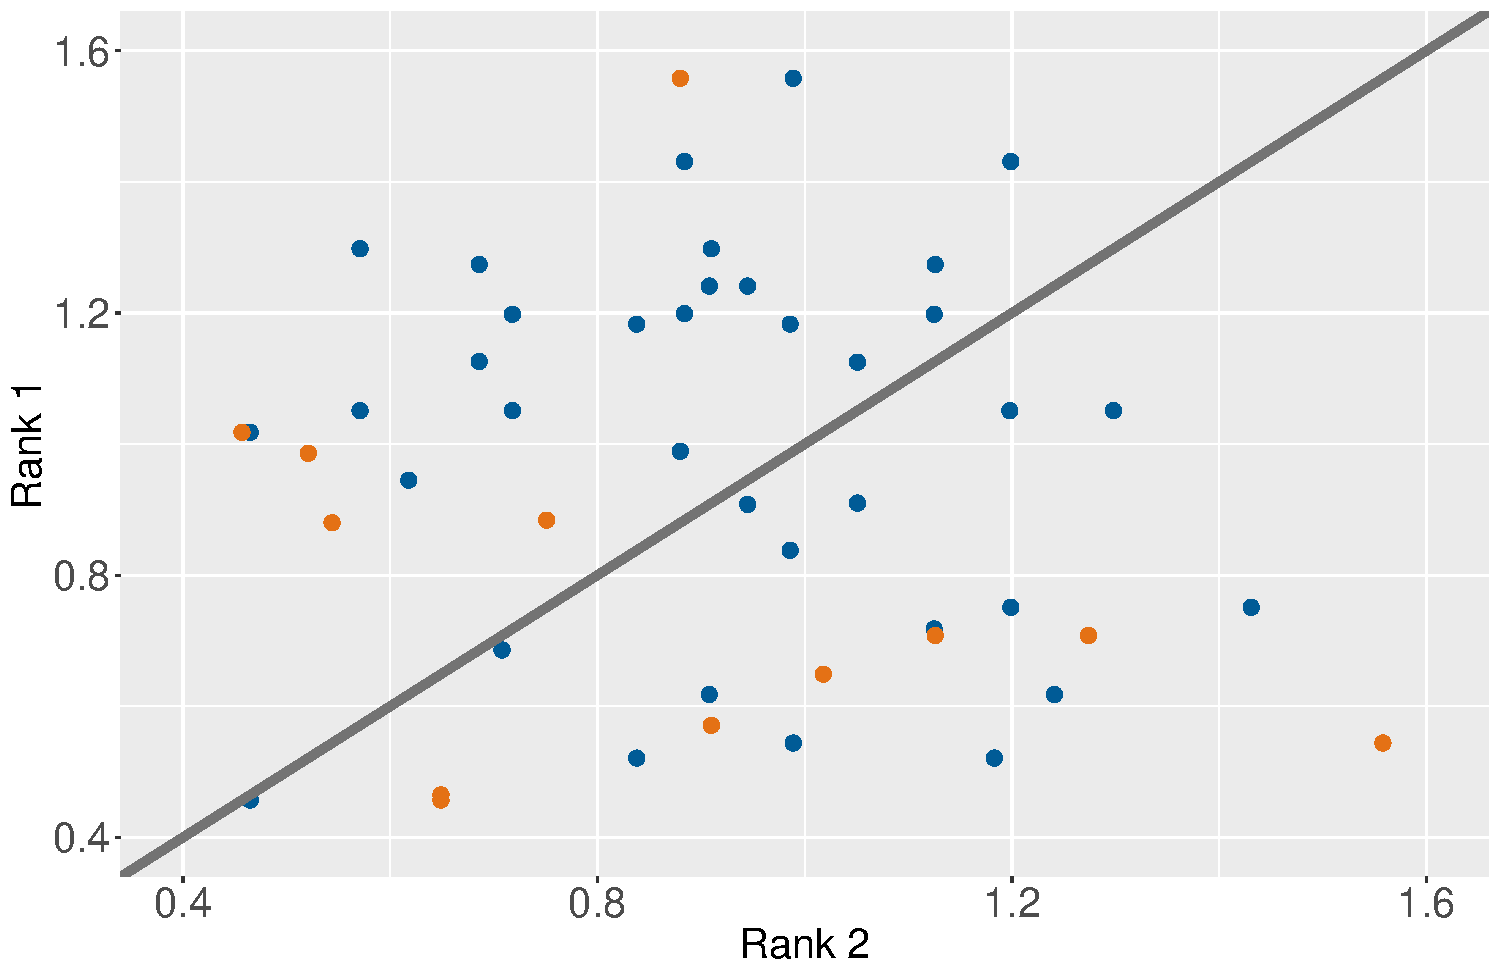
\includegraphics[scale=0.27]{ScenarioA.pdf}}~
\subfloat[Scenario B]
{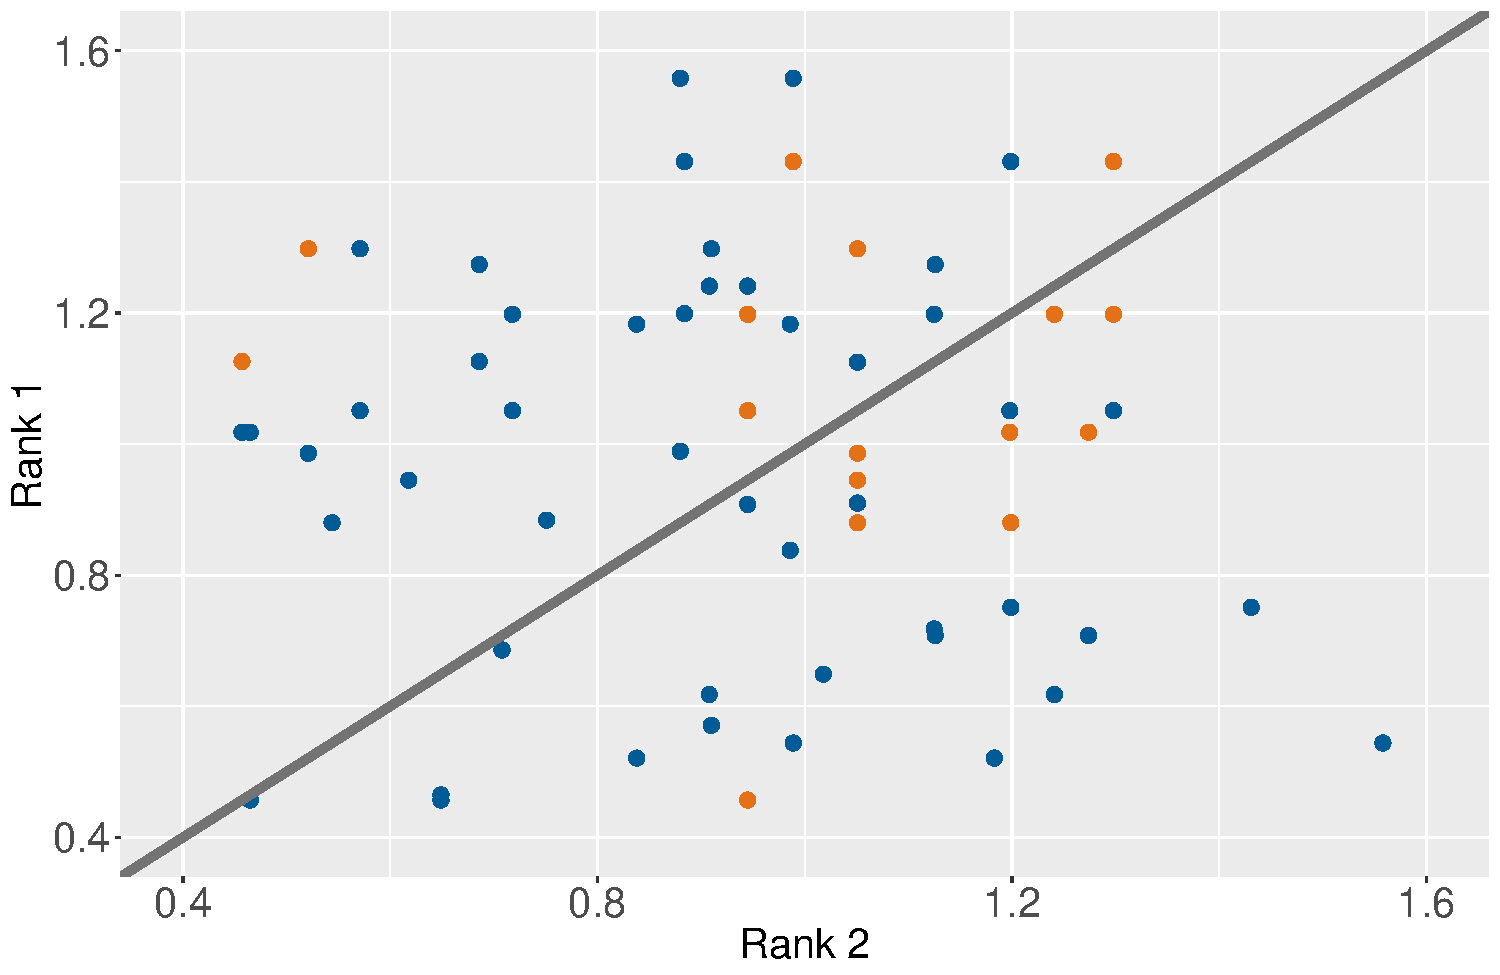
\includegraphics[scale=0.27]{ScenarioB.pdf}}\\
\centering
\subfloat[Scenario C]
{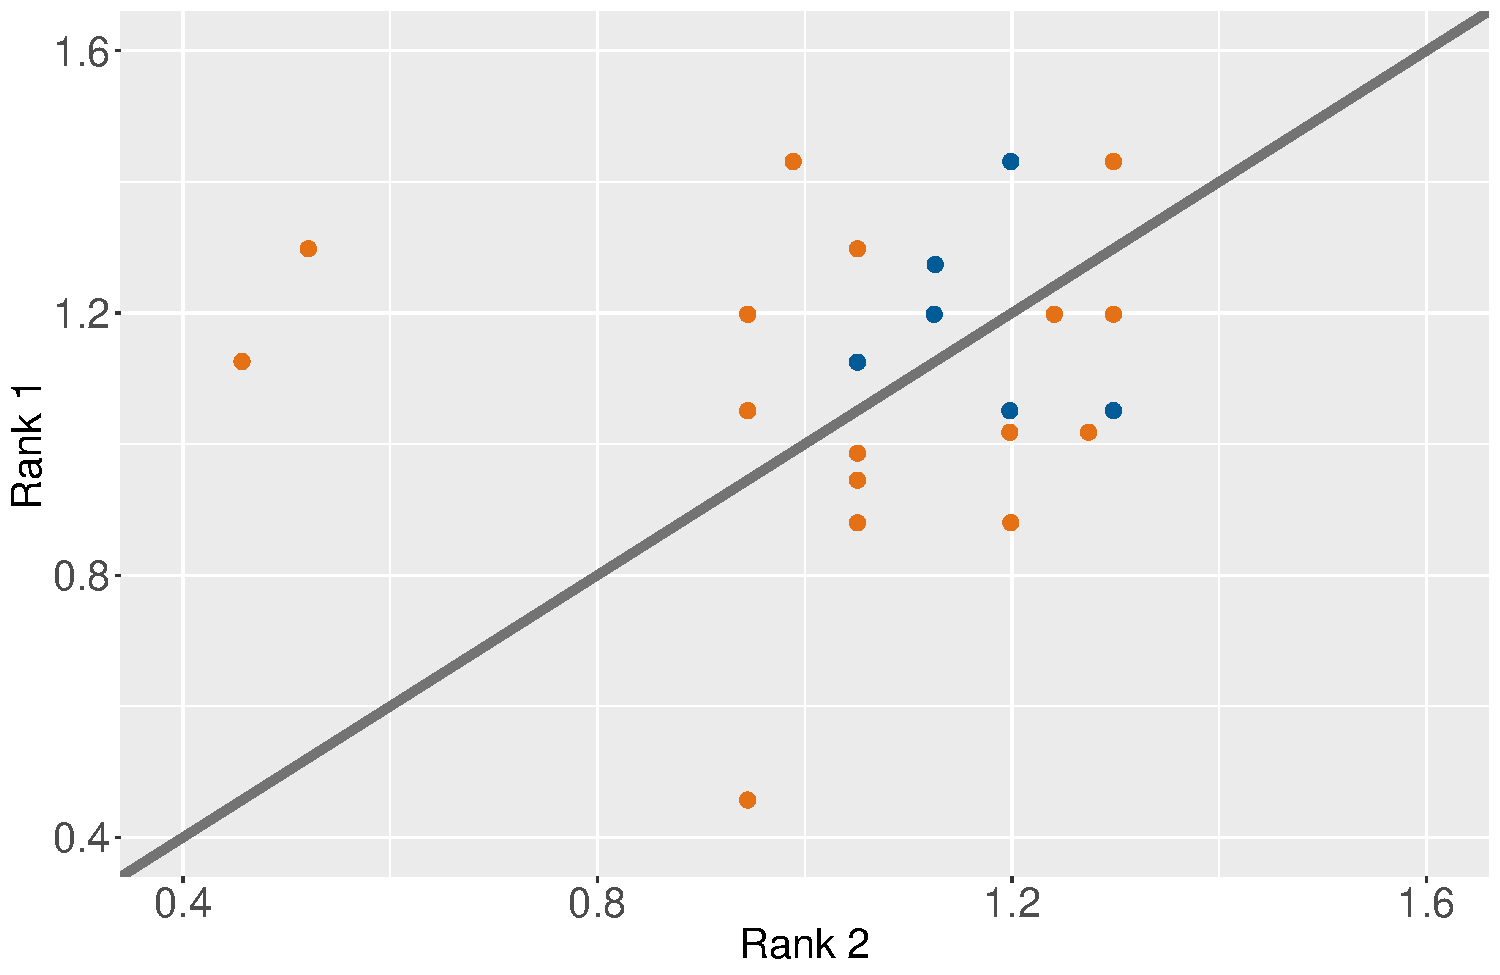
\includegraphics[scale=0.27]{ScenarioC.pdf}}
\caption{For each prediction scenarios, the values of the FIFA rankings for each match are shown in blue colour for the training set and in orange colour for the test set.}
\label{Fig1}
\end{figure}
\end{center}
%
Figure~\ref{Fig1} displays for each scenario the values for the FIFA rankings for the training set matches (blue points) and the test set matches (orange points), along with the 
line $\text{Rank }1= \text{Rank }2$, implying that the ranking difference is $w=0$. In Scenario A, the test set matches are randomly selected from the group stage, and they do not 
show any particular pattern around the line $w=0$. In scenarios B and C, test set matches belong to the knockout stage, where the teams are expected to be stronger and 
closer each other in terms of their rankings. In fact, the majority of the orange points (13 out of 16) is displayed towards the bottom right corner---higher rankings--- and closer to the line $w=0$---closer strengths. Scenario B uses more and more data to predict test set results---all the 48 group stage matches---whereas Scenario C only six matches.

Table 1 shows the accuracy in the predictions for the seven methods and the three  scenarios.  As already argued, the choice of the training and the test set can dramatically 
change the predictive performance of the ML algorithms, which over-perform statistical models only when considering a portion of the group stage to predict the remaining 
group stage matches. Instead, it is worth noting that statistical models better predict the knockout stage matches (scenario B and C), and seem to be constant across the different scenarios.

Although the example is quite simple and the dataset is too small to extract general conclusions, there are enough arguments to emphasize the paradoxical performance achieved by ML techniques. Their predictive accuracy is too much influenced by the training set 
structure, making impossible to draw conclusions about their plausibility for predicting the football World Cup. In other way said, from this simple case study we cannot openly 
falsify our ML techniques on the ground of future predictions. Conversely, Poisson models are quite stable in the three scenarios in terms of predictive accuracy, and they 
seem to learn from the group stage training set in an efficient way. We are not claiming they are better than ML tools, we are just suggesting that they seem to be less sensitive to the training set structure, and then falsifiable in a broader sense.

\begin{center}
\begin{table}
%\centering
\caption{Prediction accuracy for the selected methods, according to three prediction  scenarios.}
\begin{tabular}{|r|rrr|}
\hline 
 \emph{Train}& 75\% group  & 100\% group  & rank $>$ 1   \\ 
  \hline
\emph{Test} & 25\% group & knockout & knockout\\ 
  \hline
\emph{Random forest} & 0.67 & 0.25 & 0.44 \\ 
  \emph{Bagged CART} & 0.67 & 0.31 & 0.37  \\ 
%  bayesglm & 0.25 & 0.19 & 0.19 \\ 
  \emph{CART} & 0.58 & 0.31 & 0.19  \\ 
  \emph{MARS} & 0.58 & 0.38 & 0.49 \\ 
  \emph{NN} & 0.67 & 0.25 & 0.44  \\ 
  %Multinomial & 0.50 & 0.50 & 0.50 \\ 
  %Multinomial  & 0.42 & 0.62 & 0.62  \\ 
  \emph{Double Pois.} & 0.58 & 0.50 & 0.56  \\ 
  \emph{Biv. Pois.} & 0.58 & 0.56 & 0.56  \\ 
   \hline
\end{tabular}
%\label{tab1}
\end{table}
\end{center}
%

%Obviously it should be noted that the results presented here are only preliminary also considering the small size of the dataset here analysed. A full appreciation of the 
%different performances  is out-of the scope of the current paper and should be definitely considered for future research, also aimed  at defining a strategy for stacking models in this specific application case.

\section{Conclusions}





\bibliographystyle{chicago}
\bibliography{predbib}

\end{document}